\documentclass[10pt]{article}
\usepackage{geometry}
\geometry{a4paper} 
\usepackage{graphicx}
\usepackage{fancyhdr}
\pagestyle{fancy}
\setlength\headheight{42.88329pt}
\addtolength{\topmargin}{-0.09334pt}

\fancyhead[L]{
    \large\textbf{ICMC - Instituto de Ciências Matemáticas\\
    e da Computação} \\[0.2em]
}
\rhead{
\includegraphics[width=2.5cm]{imcmc_poggers.png}}

\graphicspath{ {./images/} }

\usepackage[portuguese]{babel}
\usepackage[section]{placeins}
\usepackage{subfigure}
\usepackage{float}

\begin{document}

\begin{center}
    \large\textbf{Disciplina: SCC0201 - Introdução à Ciência de Computação II}
    
    \large\textbf{Projeto 2}
\end{center}

\begin{tabular}{@{}ll@{}}
\textbf{Aluno:} & Alec Campos Aoki (15436800)\\
\textbf{Aluno:} & Fernando Valentim Torres (NUSP)
\end{tabular}

\vspace{0.5cm}

\textbf{1. Problema e Solução}

O trabalho consistia de comparar os métodos de ordenação BubbleSort, SelectionSort, InsertionSort, ShellSort, QuickSort, HeapSort, MergeSort, Contagem de Menores e RadixSort utilizando vetores ordenados, inversamente ordenados e aleatórios. Foram feitas comparações de tempo de execução, quantidade de trocas e quantidade de comparações.

Para tanto, implementamos cada método de ordenação e utilizamos uma struct chamada Data para armazenar a quantidade de trocas e comparações de cada algoritmo. A cada troca ou comparação, incrementamos o campo correspondente dessa struct. Além disso, nos casos teste, utilizamos somente elementos pertences ao intervalo entre 0 e a quantidade de elementos do teste (no teste de $100$ elementos, por exemplo, os números no teste vão de $0$ a $100$), para melhor padronizar os resultados obtidos.

Para melhor organizar as informações, agrupamos os algoritmos por complexidade. Sendo assim, temos os grupos:

\begin{enumerate}
  \item $O(n^2)$;
  \begin{enumerate}
    \item BubbleSort;
    \item Contagem de Menores;
    \item InsertionSort;
    \item SelectionSort;
    \item ShellSort;
  \end{enumerate}
  \item $O(n \log(n))$;
  \begin{enumerate}
    \item HeapSort;
    \item MergeSort;
    \item QuickSort;
  \end{enumerate}
  \item $O(n k)$;
  \begin{enumerate}
    \item RadixSort.
  \end{enumerate}
\end{enumerate}


\vspace{0.25cm}

\textbf{2. Tempo de Execução}

\vspace{0.5cm}

\textbf{2.1 $O(n^2)$}

\begin{figure}[H]
  \centering
  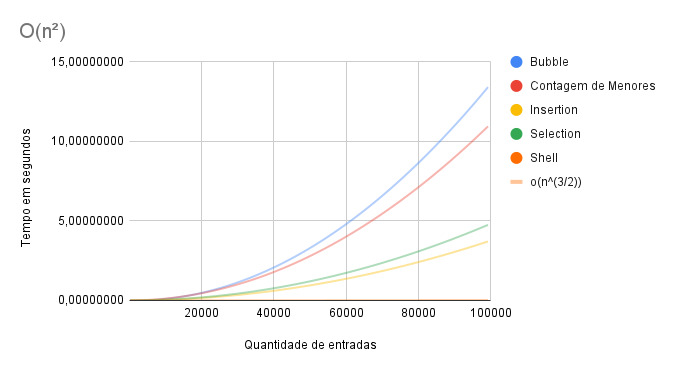
\includegraphics[width=0.8\textwidth]{TempExec1.jpg}
  \caption{Gráfico do tempo de execução dos algoritmos $O(n^2)$}
  \label{fig:1}
\end{figure}

\vspace{0.5cm}

\textbf{2.2 $O(n \log(n))$}

\begin{figure}[H]
  \centering
  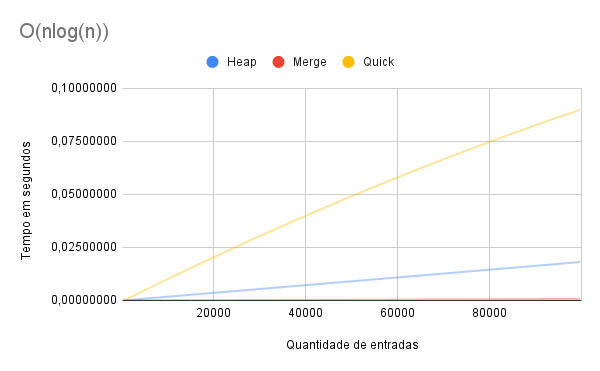
\includegraphics[width=0.7\textwidth]{TempoExec2.jpg}
  \caption{Gráfico do tempo de execução dos algoritmos $O(n \log(n))$}
  \label{fig:2}
\end{figure}

\vspace{0.5cm}

\textbf{2.3 $O(n k)$}

\begin{figure}[H]
  \centering
  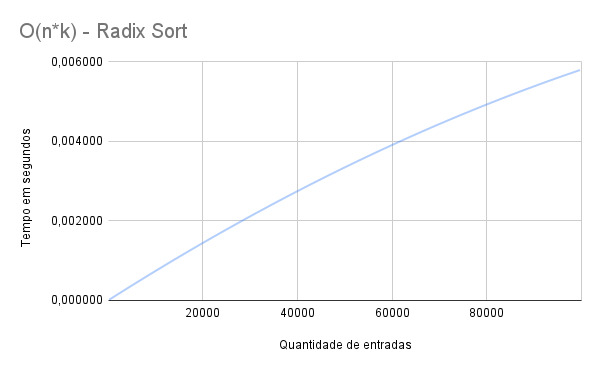
\includegraphics[width=0.7\textwidth]{TempoExec3.jpg}
  \caption{Gráfico do tempo de execução dos algoritmos $O(n k)$}
  \label{fig:3}
\end{figure}

\vspace{0.25cm}

\textbf{3. Quantidade de Comparações}

\vspace{0.5cm}

\textbf{3.1 $O(n^2)$}

\begin{table}[H]
  \parbox{.45\linewidth}{
    \centering
    \caption{Tabela de comparações BubbleSort}
    \begin{tabular}{|c|c|c|c|c|}
    \hline
    N & Ordenado & Inverso & Aleatório \\ \hline
    100 & 99 & 4950 & 4882,1 \\ \hline
    1000 & 999 & 499500 & 498700,7 \\ \hline
    10000 & 9999 & 49995000 & 49987304,1 \\ \hline
    100000 & 99999 & 4999950000 & 4999798132 \\ \hline
    \end{tabular}
  }
  \hfill
  \parbox{.45\linewidth}{
    \centering
    \caption{Tabela de comparações Contagem de Menores}
    \begin{tabular}{|c|c|c|c|c|}
    \hline
    N & Ordenado & Inverso & Aleatório \\ \hline
    100 & 4950 & 4950 & 4950 \\ \hline
    1000 & 499500 & 499500 & 499500 \\ \hline
    10000 & 49995000 & 49995000 & 49995000 \\ \hline
    100000 & 4999950000 & 4999950000 & 4999950000 \\ \hline
    \end{tabular}
  }
\end{table}

\begin{table}[H]
  \parbox{.45\linewidth}{
    \centering
    \caption{Tabela de comparações InsertionSort}
    \begin{tabular}{|c|c|c|c|c|}
    \hline
    N & Ordenado & Inverso & Aleatório \\ \hline
    100 & 99 & 4950 & 2636,3 \\ \hline
    1000 & 999 & 499500 & 249352,9 \\ \hline
    10000 & 9999 & 49995000 & 24986288,7 \\ \hline
    100000 & 99999 & 4999950000 & 2498975066 \\ \hline
    \end{tabular}
  }
  \hfill
  \parbox{.45\linewidth}{
    \centering
    \caption{Tabela de comparações SelectionSort}
    \begin{tabular}{|c|c|c|c|c|}
    \hline
    N & Ordenado & Inverso & Aleatório \\ \hline
    100 & 4950 & 4950 & 4950 \\ \hline
    1000 & 499500 & 499500 & 499500 \\ \hline
    10000 & 49995000 & 49995000 & 49995000 \\ \hline
    100000 & 4999950000 & 4999950000 & 4999950000 \\ \hline
    \end{tabular}
  }
\end{table}

\begin{table}[H]
  \centering
  \caption{Tabela de comparações ShellSort}
  \begin{tabular}{|c|c|c|c|c|}
  \hline
  N & Ordenado & Inverso & Aleatório \\ \hline
  100 & 0 & 414 & 573,7 \\ \hline
  1000 & 0 & 5188 & 11295,2 \\ \hline
  10000 & 0 & 211340 & 252463,5 \\ \hline
  100000 & 0 & 18184250 & 11965729,8 \\ \hline
  \end{tabular}
\end{table}

\vspace{0.5cm}

\textbf{3.2 $O(n \log(n))$}

\begin{table}[H]
  \parbox{.45\linewidth}{
    \centering
    \caption{Tabela de comparações HeapSort}
    \begin{tabular}{|c|c|c|c|c|}
    \hline
    N & Ordenado & Inverso & Aleatório \\ \hline
    100 & 1380 & 1132 & 1262,2 \\ \hline
    1000 & 20416 & 17632 & 19143,2 \\ \hline
    10000 & 273912 & 243392 & 258448,2 \\ \hline
    100000 & 3401708 & 3094868 & 3249879,6 \\ \hline
    \end{tabular}
  }
  \hfill
  \parbox{.45\linewidth}{
    \centering
    \caption{Tabela de comparações MergeSort}
    \begin{tabular}{|c|c|c|c|c|}
    \hline
    N & Ordenado & Inverso & Aleatório \\ \hline
    100 & 99 & 102 & 188,9 \\ \hline
    1000 & 999 & 1001 & 1981,3 \\ \hline
    10000 & 9999 & 10005 & 19977,4 \\ \hline
    100000 & 99999 & 100006 & 199975,4 \\ \hline
    \end{tabular}
  }
\end{table}

\begin{table}[H]
  \centering
  \caption{Tabela de comparações QuickSort}
  \begin{tabular}{|c|c|c|c|c|}
  \hline
  N & Ordenado & Inverso & Aleatório \\ \hline
  100 & 756 & 1417 & 873,9 \\ \hline
  1000 & 10814 & 102188 & 12786,1 \\ \hline
  10000 & 141660 & 9744569 & 178437,5 \\ \hline
  100000 & 1747098 & 968505521 & 2232338,6 \\ \hline
  \end{tabular}
\end{table}

\vspace{0.5cm}

\textbf{3.3 $O(n k)$}

\begin{table}[H]
  \centering
  \caption{Tabela de comparações RadixSort}
  \begin{tabular}{|c|c|c|c|c|}
  \hline
  N & Ordenado & Inverso & Aleatório \\ \hline
  100 & 100 & 100 & 100 \\ \hline
  1000 & 1000 & 1000 & 1000 \\ \hline
  10000 & 10000 & 10000 & 10000 \\ \hline
  100000 & 100000 & 100000 & 100000 \\ \hline
  \end{tabular}
\end{table}

\vspace{0.25cm}

\textbf{4. Movimentações}

\vspace{0.5cm}

\textbf{4.1 $O(n^2)$}

\begin{table}[H]
  \parbox{.45\linewidth}{
    \centering
    \caption{Tabela de trocas BubbleSort}
    \begin{tabular}{|c|c|c|c|c|}
    \hline
    N & Ordenado & Inverso & Aleatório \\ \hline
    100 & 0 & 4950 & 2542,9 \\ \hline
    1000 & 0 & 499500 & 248360,4 \\ \hline
    10000 & 0 & 49995000 & 24976298,5 \\ \hline
    100000 & 0 & 4999950000 & 2271704616 \\ \hline
    \end{tabular}
  }
  \hfill
  \parbox{.45\linewidth}{
    \centering
    \caption{Tabela de trocas Contagem de Menores}
    \begin{tabular}{|c|c|c|c|c|}
    \hline
    N & Ordenado & Inverso & Aleatório \\ \hline
    100 & 100 & 100 & 100 \\ \hline
    1000 & 1000 & 1000 & 1000 \\ \hline
    10000 & 10000 & 10000 & 10000 \\ \hline
    100000 & 100000 & 100000 & 100000 \\ \hline
    \end{tabular}
  }
\end{table}

\begin{table}[H]
  \parbox{.45\linewidth}{
    \centering
    \caption{Tabela de trocas InsertionSort}
    \begin{tabular}{|c|c|c|c|c|}
    \hline
    N & Ordenado & Inverso & Aleatório \\ \hline
    100 & 99 & 5049 & 2641,9 \\ \hline
    1000 & 999 & 500499 & 249359,4 \\ \hline
    10000 & 9999 & 50004999 & 24986297,5 \\ \hline
    100000 & 99999 & 5000049999 & 2498975077 \\ \hline
    \end{tabular}
  }
  \hfill
  \parbox{.45\linewidth}{
    \centering
    \caption{Tabela de trocas SelectionSort}
    \begin{tabular}{|c|c|c|c|c|}
    \hline
    N & Ordenado & Inverso & Aleatório \\ \hline
    100 & 0 & 50 & 94,7 \\ \hline
    1000 & 0 & 500 & 993,6 \\ \hline
    10000 & 0 & 5000 & 9991,5 \\ \hline
    100000 & 0 & 50000 & 99987,8 \\ \hline
    \end{tabular}
  }
\end{table}

\begin{table}[H]
  \centering
  \caption{Tabela de trocas ShellSort}
  \begin{tabular}{|c|c|c|c|c|}
  \hline
  N & Ordenado & Inverso & Aleatório \\ \hline
  100 & 291 & 705 & 864,7 \\ \hline
  1000 & 4610 & 9798 & 15905,2 \\ \hline
  10000 & 49610 & 260950 & 302073,5 \\ \hline
  100000 & 499610 & 18683860 & 12465339,8 \\ \hline
  \end{tabular}
\end{table}

\vspace{0.5cm}

\textbf{4.2 $O(n \log(n))$}

\begin{table}[H]
  \parbox{.45\linewidth}{
    \centering
    \caption{Tabela de trocas HeapSort}
    \begin{tabular}{|c|c|c|c|c|}
    \hline
    N & Ordenado & Inverso & Aleatório \\ \hline
    100 & 640 & 516 & 581,1 \\ \hline
    1000 & 9708 & 8316 & 9071,6 \\ \hline
    10000 & 131956 & 116696 & 124224,1 \\ \hline
    100000 & 1650854 & 1497434 & 1574939,8 \\ \hline
    \end{tabular}
  }
  \hfill
  \parbox{.45\linewidth}{
    \centering
    \caption{Tabela de trocas MergeSort}
    \begin{tabular}{|c|c|c|c|c|}
    \hline
    N & Ordenado & Inverso & Aleatório \\ \hline
    100 & 201 & 201 & 201 \\ \hline
    1000 & 2000 & 2000 & 2000 \\ \hline
    10000 & 20004 & 20004 & 20004 \\ \hline
    100000 & 200005 & 200005 & 200005 \\ \hline
    \end{tabular}
  }
\end{table}

\begin{table}[H]
  \centering
  \caption{Tabela de trocas QuickSort}
  \begin{tabular}{|c|c|c|c|c|}
  \hline
  N & Ordenado & Inverso & Aleatório \\ \hline
  100 & 424 & 1179 & 482 \\ \hline
  1000 & 5840 & 99206 & 6731,8 \\ \hline
  10000 & 75580 & 9709257 & 93351,2 \\ \hline
  100000 & 919107 & 968096337 & 1164047,7 \\ \hline
  \end{tabular}
\end{table}

\vspace{0.5cm}

\textbf{4.3 $O(n k)$}

\begin{table}[H]
  \centering
  \caption{Tabela de trocas RadixSort}
  \begin{tabular}{|c|c|c|c|c|}
  \hline
  N & Ordenado & Inverso & Aleatório \\ \hline
  100 & 300 & 300 & 300 \\ \hline
  1000 & 4000 & 4000 & 4000 \\ \hline
  10000 & 50000 & 50000 & 50000 \\ \hline
  100000 & 600000 & 600000 & 600000 \\ \hline
  \end{tabular}
\end{table}

\vspace{0.25cm}

\textbf{5. Análise dos Resultados}



\vspace{0.25cm}

\end{document}